\chapter{Nuova architettura}
\label{cha:nuova_architettura}

In seguito alla scelta del framework da utilizzare, i passaggi successivi per iniziare
ad utilizzare il nuovo sistema sono: creare una nuova infrastruttura (macchina virtuale
dedicata) per Airflow, portare la vecchia implementazione sulla nuova infrastruttura
e scegliere una strategia per il rilascio in produzione. Nelle sezioni seguenti
verranno discusse dettagliatamente le fasi di migrazione e alcune decisioni
implementative.

\begin{figure}[htbp]
  \centering
  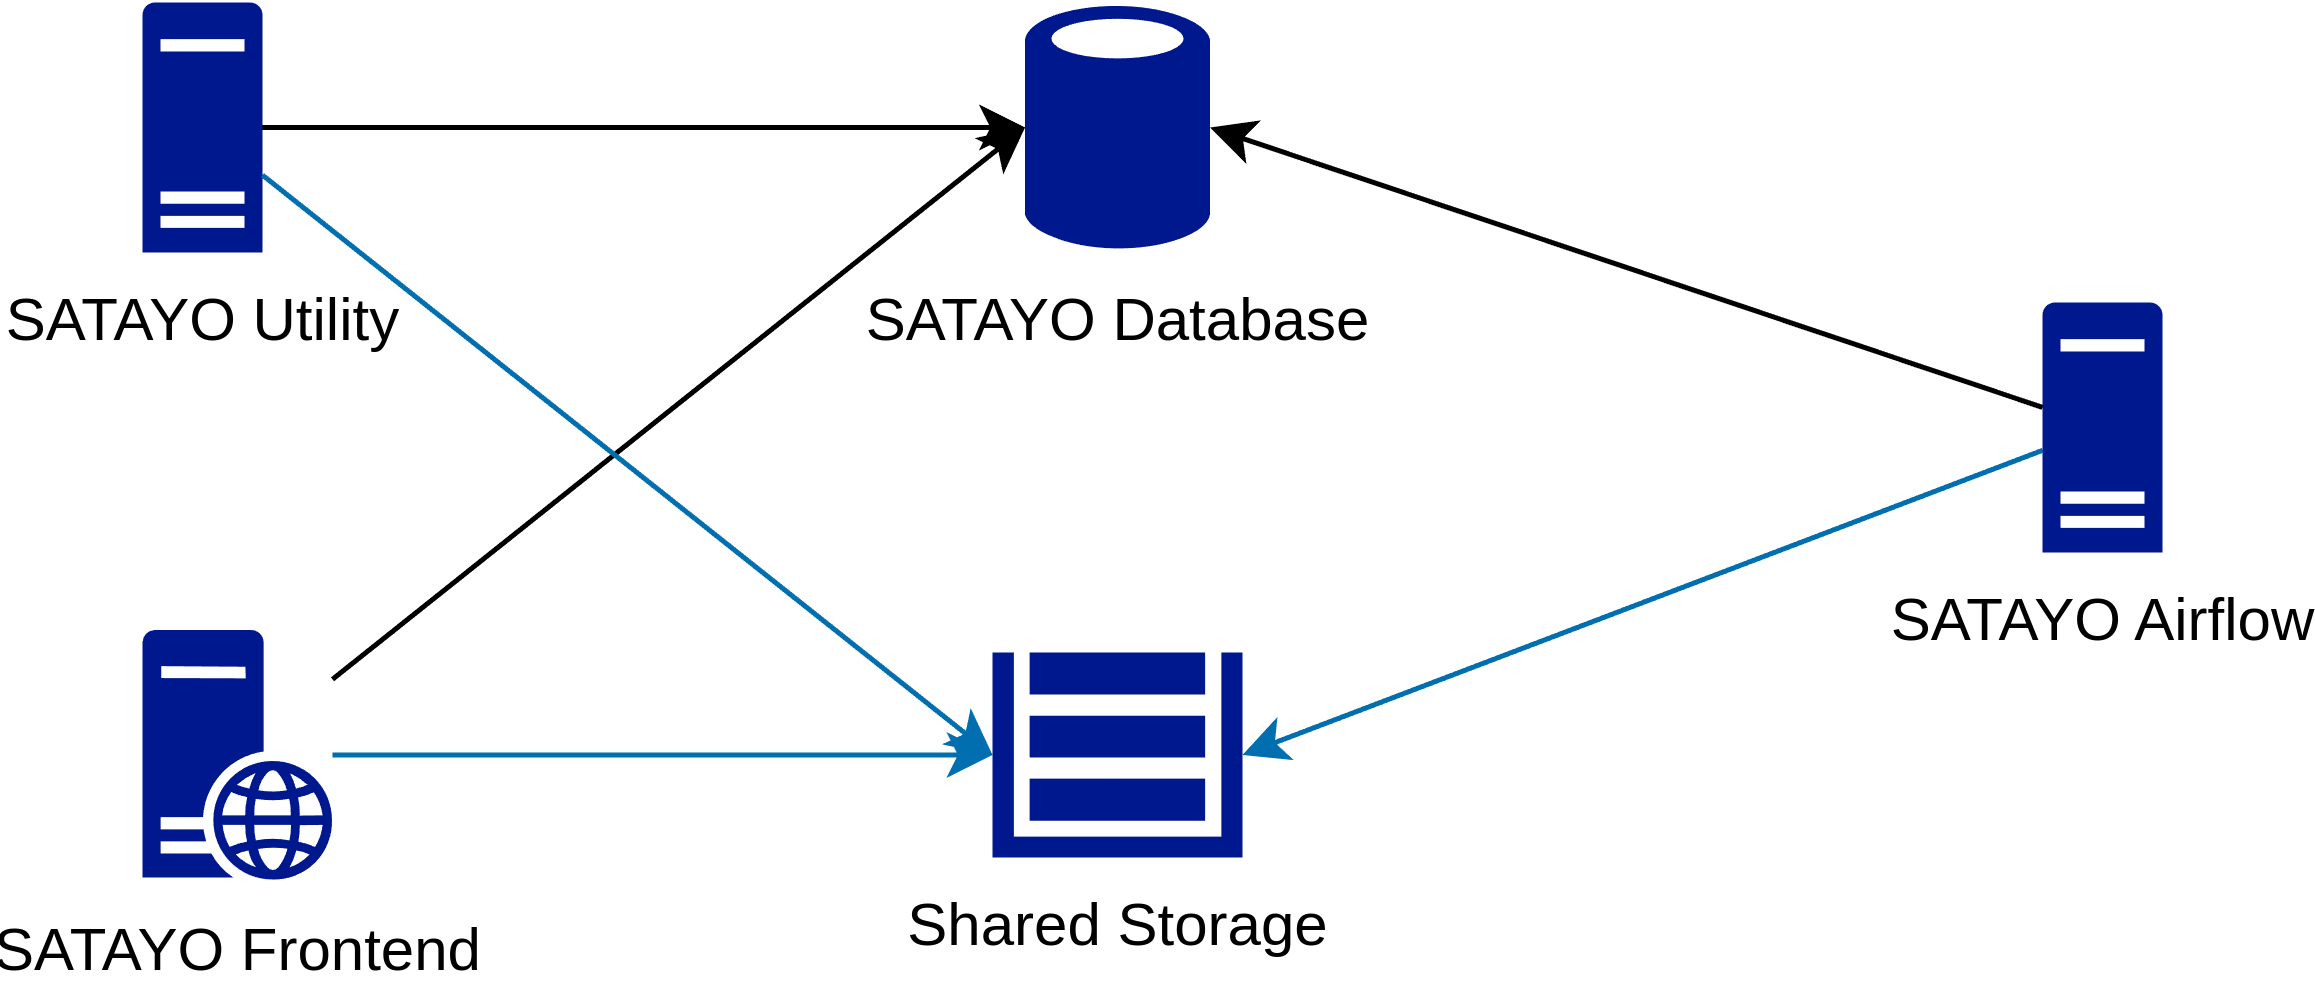
\includegraphics[width=.6\linewidth]{images/SATAYO_infrastructure_new.png}
  \caption{Nuova infrastruttura di SATAYO}
  \label{fig:infra_new}
\end{figure}

\section{Implementazione e Containerizzazione}
\label{sec:impl_container}

Dopo una prima analisi dei metodi di deployment messi a disposizione da Airflow,
è stato deciso di procedere inizialmente con l'utilizzo di un'immagine Docker\cite{docker}
istanziata su più container gestiti tramite Docker Compose. Nonostante questo approccio
sia sconsigliato dalla documentazione, che incita ad usare Kubernetes per gli
ambienti di produzione, è stato il modo più veloce per ottenere un'ambiente funzionante.
Sebbene possa sembrare, in primo luogo, che questa decisione porti ad un
ulteriore debito tecnico, non è assolutamente il caso. Il \texttt{Dockerfile} che
è stato scritto per questa implementazione, infatti, può essere utilizzato anche
per il deployment su Kubernetes.

Il \texttt{Dockerfile} descrivente l'immagine utilizzata, è stato implementato utilizzando
come base l'immagine ufficiale di Airflow \texttt{apache/airflow} e aggiungendo
tutte le dipendenze e tool OSINT utilizzati dalle fasi di SATAYO. Questo ha permesso
di semplificare l'implementazione delle fasi, in quanto non deve più essere
eseguito un controllo a tempo di esecuzione per verificare la presenza del tool
da eseguire. Le altre modifiche effettuate sul codice della vecchia implementazione
delle task, consultabile in \ref{lst:task-impl-old}, sono state: rimuovere il
controllo sul \texttt{id\_tool\_progress}, in quanto su Airflow l'esecuzione
della task avviene soltanto dopo che le sue dipendenze sono state risolte, non necessitando
quindi di controlli secondari all'interno della funzione stessa; aggiungere il
decoratore \texttt{@satayo\_task} all'inizio della definizione di ogni fase, il
quale ha la funzione di provvedere gli argomenti in modo tale che la nuova
implementazione sia compatibile con quella vecchia. Queste modifiche si possono osservare
nel codice nuovo \ref{lst:task-impl-new}, in cui viene direttamente eseguito il
corpo della fase.

Come precedentemente riportato, attualmente Airflow è utilizzato tramite Docker Compose,
è quindi in funzione su una macchina singola e l'infrastruttura è come riportato
in figura \ref{fig:infra_new}.

\pagebreak
\lstinputlisting[language=Python, caption=Esempio della precedente implementazione
di una fase di SATAYO, label=lst:task-impl-old]{listings/task-old.py}

\lstinputlisting[language=Python, caption=Esempio della nuova implementazione della
medesima fase, label=lst:task-impl-new]{listings/task-new.py}

\section{Retrocompatibilità}
\label{sec:retrocompatibility}

Per permettere una corretta integrazione del nuovo sistema all'interno di quello
corrente, mantenendo tutte le funzionalità presenti, è necessario continuare ad utilizzare
alcune funzionalità che potrebbero essere deprecate e sostituite interamente da Airflow.
In particolare occorre mantenere l'uso del \texttt{tool\_progress}, descritto
nella sezione \ref{sub:db:tasks}, in quanto questo viene utilizzato per calcolare
la data di ultima esecuzione di una determinata fase di SATAYO e per individuare
la fase che ha recuperato una certa evidenza. Per evitare la duplicazione di
codice è stato deciso di implementare questa funzionalità all'interno del
decoratore \texttt{@satayo\_task} (scritto utilizzando una classe Python) tramite
le due funzioni \texttt{pre\_task} e \texttt{post\_task}. L'implementazione
dettagliata è riportata in \ref{lst:retro}, si può notare come, nella prima
funzione, eseguita prima dell'esecuzione della task, venga utilizzato un \texttt{host\_id}
dedicato per le esecuzioni su Airflow, e sia creato un \texttt{tool\_progress} che
riporta le informazioni dell'esecuzione delle task come se venissero eseguite sul
sistema precedente. Nella seconda funzione, eseguita successivamente alla task,
viene invece impostata la data e lo stato di termine di essa. Per il caso di errore
di esecuzione viene chiamata una funzione di callback, presente tra gli
argomenti della task Airflow, che imposta il \texttt{tool\_progress} in stato di
errore.

Un'altra funzionalità riportata momentaneamente è la possibilità di salvare
certi messaggi di log all'interno del database. Questo è stato fatto per avere visibilità
su certi errori che non terminerebbero con errore la task, ma sarebbe comunque
opportuno controllare in caso si presentassero.

Infine è risultato necessario implementare anche un modo per delegare l'esecuzione
di alcune fasi al sistema vecchio, in quanto necessitanti di prerequisiti infrastrutturali
quali VPN o Proxy al momento non implementati all'interno del sistema basato su Airflow.
Ciò è stato ottenuto dividendo l'esecuzione in due parti: la prima task svolge la
funzionalità di creare un \textit{tool\_progress} e assegnarlo ad una macchina
Robot, la seconda è un \textit{Sensor} di Airflow che controlla con intervalli
regolari se la fase in questione è terminata e continua l'esecuzione del DAG in
base al risultato (successo continua l'esecuzione, errore viene interrotta e
notificata sulle dashboard descritte al punto \ref{sec:monitoraggio}).

\lstinputlisting[language=Python, caption={Implementazione delle funzioni di \texttt{@satayo\_task} che permettono la retrocompatibilità},
label=lst:retro]{listings/retrocompatibility-funcs.py}

\section{Ricerche schedulate}
\label{sec:schedulate}

\lstinputlisting[language=Python, caption={Funzione che calcola una schedulazione pseudo randomica per ogni dominio},
label=lst:schedule]{listings/schedule-generation.py}

Una delle funzionalità più interessanti di SATAYO per un cliente, è il monitoraggio
continuo della propria esposizione online. Per ottenere questo risultato è
essenziale eseguire determinate fasi secondo una schedulazione predefinita; nel dettaglio,
ci saranno delle task che devono essere eseguite giornalmente, settimanalmente o
ogni due settimane. Ciò è implementato dalle seguenti operazioni: viene eseguita
una query per collezionare la lista di domini da monitorare; da questa lista
vengono generati dinamicamente 3 DAG per ogni dominio, ognuno di essi contenente
le task da eseguire rispettivamente ogni giorno, settimana o due settimane. Per distribuire
equamente nel tempo le esecuzioni dei DAG settimanali e bisettimanali viene utilizzata
la funzione riportata in \ref{lst:schedule}. Il funzionamento di quest'ultima si
basa sul fatto che un PRNG (PseudoRandom Number Generator)\cite{py-random},
inizializzato con lo stesso \texttt{seed}, produrrà la medesima sequenza di
numeri. Utilizzando quindi come \texttt{seed} il dominio da analizzare, i DAG riferiti
ad esso verranno eseguiti con intervalli regolari e in giorni costanti. Per i
DAG settimanali verrà scelto un giorno casuale della settimana, mentre per quelli
bisettimanali verranno casualmente scelti due giorni del mese distanti 14 giorni.

\section{Nuove ricerche}
\label{sec:nuove}

\begin{figure}[htbp]
  \centering
  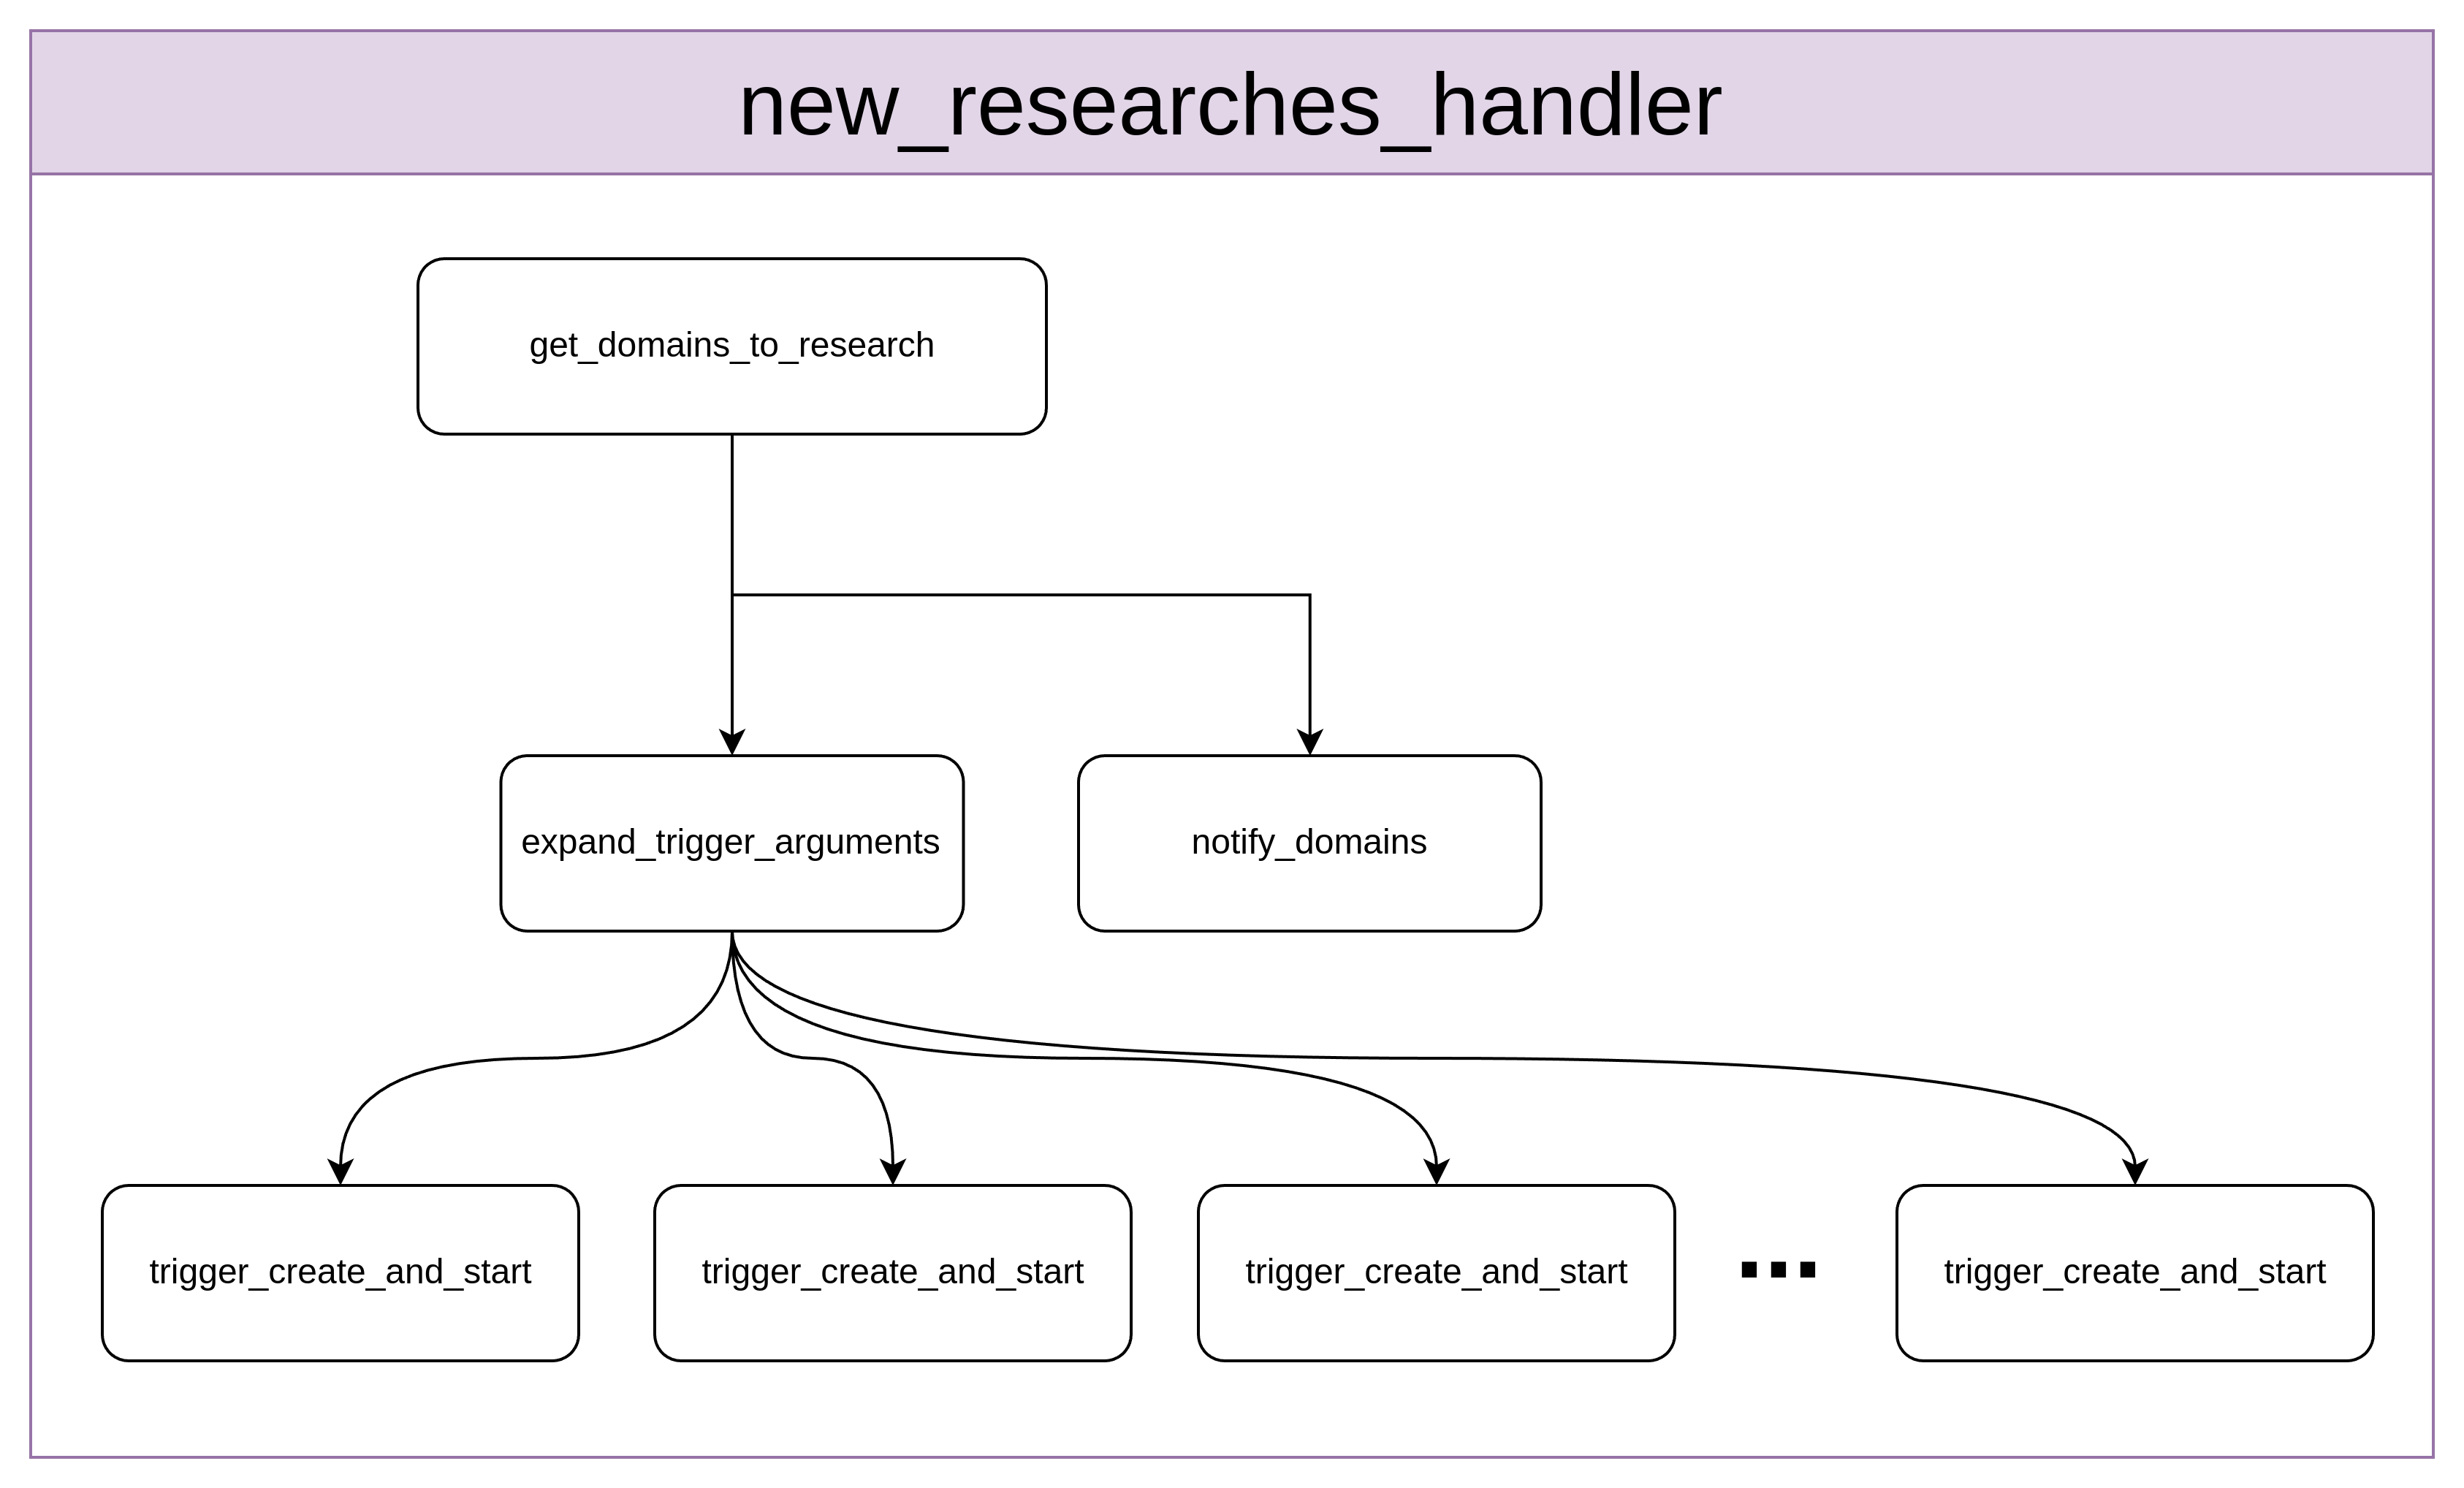
\includegraphics[width=.6\linewidth]{images/new_research_handler.png}
  \caption{DAG per gestire la schedulazione automatica di nuove ricerche}
  \label{fig:new-hanlder}
\end{figure}

Sebbene ci sia un monitoraggio continuo degli asset principali e più pericolosi,
in quanto più probabilmente utilizzati per organizzare campagne di Phishing, le fasi
ricorrenti non coprono tutto il perimetro dei clienti. Per questo è necessario
eseguire in modo ricorrente anche i controlli più pesanti e lunghi, ovviamente con
minore frequenza. Dato il più alto carico computazionale, è stato scelto di utilizzare
un approccio più controllato per schedulare i DAG delle nuove ricerche \texttt{start\_new\_research}.
Nel dettaglio è presente un DAG \texttt{new\_research\_handler} che ha il
compito di: collezionare i domini di cui eseguire la nuova ricerca, notificare
tali domini prima dell'inizio dell'esecuzione delle ricerche e creare ed avviare
le nuove ricerche stesse. Questo DAG viene eseguito tre volte al giorno in orario
lavorativo, in quanto i DAG ricorrenti vengono eseguiti di notte, in modo tale di
poter intervenire in caso di malfunzionamenti. Analizzando il DAG riportato in
figura \ref{fig:new-hanlder}, si può notare la presenza delle seguenti task:

\begin{itemize}
  \item \textbf{get\_domains\_to\_research:} la quale raccoglie in base all'età
    della ricerca e ad altri parametri i domini per cui creare una nuova ricerca.
    Colleziona inoltre anche i domini di cui è stata richiesta manualmente l'esecuzione
    di una ricerca completa. Questa task genera una lista di domini che verrà
    passata alla task successiva;

  \item \textbf{notify\_domains:} implementa un sistema di notifica tramite
    messaggio di notifica con Bot Telegram\footnote{\url{https://core.telegram.org/bots}},
    questo permette di avere una visione immediata e di alto livello sulle nuove
    ricerche che stanno per essere eseguite. Questo è importante perché, come
    specificato precedentemente, si tratta di un'operazione importante che, in
    caso di malfunzionamenti potrebbe portare a gravi ripercussioni;

  \item \textbf{expand\_trigger\_arguments:} è una task di natura puramente
    implementativa, serve cioè soltanto a convertire la lista di domini fornita da
    \texttt{get\_domains\_to\_research} in un formato tale da essere compatibile
    con le task successive. Viene quindi, per ogni dominio, creato un \texttt{trigger\_run\_id}
    e un oggetto \texttt{conf} che verranno passati alla task successiva, la
    quale avrà effettivamente il compito di avviare le nuove ricerche;

  \item \textbf{trigger\_create\_and\_start:} ha il compito fondamentale di
    eseguire il DAG responsabile della creazione della nuova ricerca sul
    database, \texttt{create\_and\_start\_new\_research}, la quale viene eseguita
    importando tutte le informazioni utili dalla ricerca precedente, e dell'avvio
    vero e proprio del DAG \texttt{start\_new\_research} incaricato di eseguire effettivamente
    tutte le task necessarie a svolgere una nuova ricerca. Questa task viene
    generata in modo dinamico in base agli oggetti presenti nella lista generata
    allo step precedente che corrispondono al numero di domini per cui
    istanziare una nuova ricerca. In seguito, ciascuna Task Instance creerà una
    DAG Run differente, del medesimo DAG, per ogni oggetto nella lista.
\end{itemize}

\section{Task di sistema}
\label{sec:sistema}

Per una corretta integrazione con il vecchio sistema di SATAYO è stato necessario
creare delle routine di sincronizzazione. In particolare viene riportata una
descrizione della task \texttt{satayo\_tp\_sync}, responsabile della
sincronizzazione dello stato dei tool\_progress sul database di SATAYO con lo
stato effettivo presente su Airflow. La task in questione è necessaria in quanto
possono verificarsi dei casi in cui le funzioni \texttt{pre\_task} e \texttt{post\_task}
descritte al punto \ref{sec:retrocompatibility} non vengano eseguite correttamente.
I casi in questione sono principalmente interventi manuali sullo stato delle
task. Per evitare l'inserimento di logiche inutilmente complesse all'interno della
definizione delle task è stata implementata una task dedicata, eseguita ogni 10
minuti, che gestisce i seguenti due casi:

\begin{itemize}
  \item se viene trovato un tool\_progress che individua la task come in esecuzione
    e, al contrario, all'interno di Airflow tale task non ha lo stato \textit{running},
    essa viene impostata, all'interno del db di SATAYO come \textit{failed};

  \item al contrario invece, se all'interno della tabella dei tool\_progress
    viene trovata una fase in stato \textit{failed}, ma all'interno di Airflow
    essa è riportata con lo stato \textit{success}, ne viene cambiato lo stato
    sul database e impostato anch'esso a \textit{success}. Questo comportamento
    capita spesso nel caso in cui una task, terminata in errore, venga eseguita
    un secondo momento, creando un ulteriore tool\_progress.
\end{itemize}

A seguito di entrambe le precedenti azioni, vengono inoltre inseriti dei messaggi
di log all'interno della tabella \texttt{log} del database di SATAYO, per permettere
una migliore visibilità delle azioni della routine.

\section{Testing e rilascio in produzione}
\label{sec:deployment}

Avendo a disposizione un ambiente di test limitato è stato deciso di utilizzare
la strategia di rilascio \textit{Canary Deployment Strategy}\cite{humble2010continuous}.
Il motivo principale della presenza di un contesto di test particolarmente ridotto
è la natura del progetto. Molte funzionalità di SATAYO infatti si basano sul
fatto di avere a disposizione lo storico delle informazioni collezionate sui
domini in analisi. Questo può essere simulato in un ambiente di test, ma non è
possibile riportare le informazioni come se fosse un environment di produzione
vero e proprio. Un secondo problema, dettato dalla complessità del progetto, è la
quantità ingente di fasi, ricorrenti e non, eseguite in produzione. Questo non
permette infatti di utilizzare ambienti di test per fare prove di carico senza
utilizzare un'infrastruttura identica a quella di produzione.

Per validare quindi i risultati ottenuti dalla nuova implementazione è stata
utilizzata la strategia \textit{A/B Testing}\cite{QUIN2024112011}, che consiste nell'eseguire
la stessa operazione su due versioni diverse della stessa applicazione e confrontare
i risultati. In questo caso sono state eseguite delle ricerche complete sullo
stesso dominio, su entrambe le infrastrutture e sono stati paragonati, alla
vecchia implementazione, il numero e la qualità dei risultati ottenuti dalla nuova.

Infine è stata eseguita la procedura di \textit{Canary Deployment} menzionata
prima per migrare la vecchia versione a quella nuova. Il \textit{Canary
Deployment} consiste nel migrare gradualmente il carico di lavoro da una istanza
ad un'altra, avente una versione più recente del software. Nel caso specifico di
SATAYO sono state inizialmente migrate le fasi ricorrenti, procedendo con batch di
circa 100 domini alla settimana. Una volta terminata la migrazione delle fasi
schedulate, si è passati alla migrazione delle nuove ricerche, che inizialmente
venivano eseguite manualmente sulla nuova piattaforma, ed in seguito, a
migrazione completa, sono state automatizzate.

\section{Monitoraggio}
\label{sec:monitoraggio}

Ultimo sviluppo fondamentale per ottenere un sistema pronto al rilascio in
produzione è stata l'implementazione di un sistema di monitoraggio. I requisiti di
un tale sistema sono: una visione di insieme dello stato di esecuzione dei DAG e
altre interfacce che presentino informazioni relative a tutto il sistema con
maggiori dettagli e granularità. Per l'implementazione delle dashboard in questione
è stato utilizzato il modulo di NetEye \textit{ITOA} (IT Operations Analytics), il
quale è realizzato utilizzando il software di visualizzazione Open source \textbf{Grafana}\footnote{\url{https://grafana.com/grafana/}}.
Nello specifico è stata realizzata una dashboard che include tutte le
informazioni importanti riguardanti lo stato del sistema, la quale è presentata in
figura \textbf{\textit{X}}. In questa visualizzazione sono presenti informazioni
quali: il numero di fasi in errore, divise per tipologia (Airflow o Robot); il
\textit{tempo macchina} utilizzato, inteso come tempo utilizzato dall'esecuzione
delle task considerato sul numero massimo di task eseguibili in parallelo; le fasi
in esecuzione e altre informazioni riguardanti le code dei due sistemi. Una
seconda dashboard di rilievo è sicuramente la \textit{Airflow Failed Management}\ref{fig:errors_dash},
utilizzata appunto per gestire e rilanciare le fasi che hanno prodotto errori di
esecuzione. In questa dashboard è possibile notare una visualizzazione generale,
divisa per tipologia di DAG a cui appartengono le task in errore e un'aggregazione
del numero di fasi diverse che hanno prodotto errori. Al centro è presente una
tabella con tutti gli errori da gestire e link rapidi alle rispettive pagine di
log. Entrambe le dashboard hanno associato ad ogni pannello un link rapido alla pagina
inerente all'informazione mostrata. Oltre a queste sono presenti anche altre
visualizzazioni quali: un'aggregazione di statistiche di esecuzione delle fasi,
monitoraggio delle API utilizzate dai vari servizi a pagamento sui quali si basa
SATAYO e storico dell'utilizzo di \textit{tempo macchina}.

\textbf{\textit{INSERIRE DASHBOARD PRINCIPALE DI SATAYO, X}}

\begin{figure}[htbp]
  \centering
  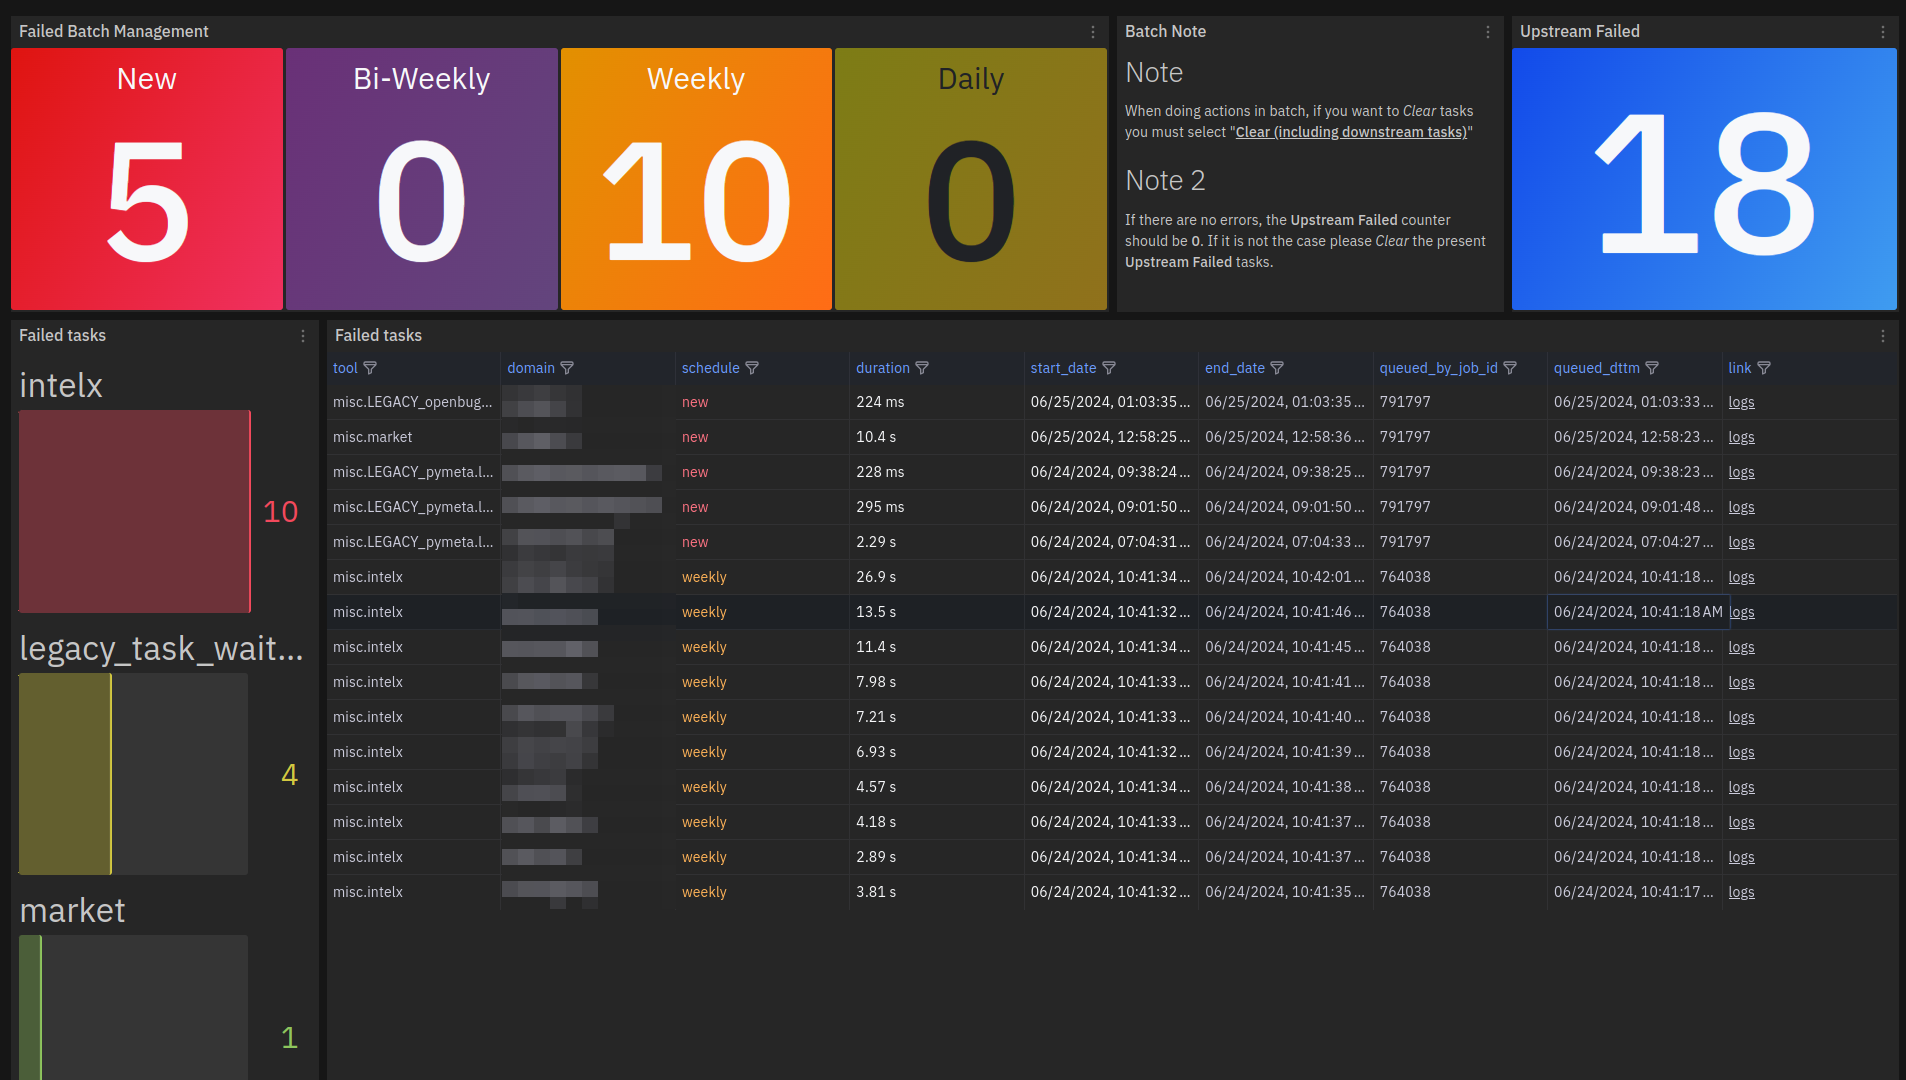
\includegraphics[width=.8\linewidth]{images/SATAYO_errors_dashboard.png}
  \caption{Dashboard di gestione errori di SATAYO}
  \label{fig:errors_dash}
\end{figure}